\chapter{مدل‌سازی تعامل شئ}\label{senario-table}
برای مدل‌‌سازی تعامل شئ، ۵ گام وجود دارد که به ترتیب باید انجام شوند:
\begin{enumerate}
	\item
	جمع‌آوری اطلاعات درباره‌ی فرایند‌های کسب‌وکار موجود 
	\item 
	تبیین سناریو‌هایی برای گام‌های غیربدیهی از مورد کاربرد‌های گسترده
	\item 
	ساخت جدول سناریو
	\item 
	استنتاج نمودار توالی از جداول سناریو
	\item 
	مرور مدل‌های تعامل شئ
\end{enumerate}
که در ادامه، با شناختی که از کسب‌وکار تا به اینجای کار پیدا کرده‌ایم، ۷ سناریو و جداول مربوطه در کنار آن نمودار توالی را نشان داده‌ایم.


\clearpage
\section{سناریو و مدل تعامل شئ برای گام 6 از \uc{14}}
\subsection{سناریو تعامل شئ برای \say{ثبت کردن آگهی}}
\setcounter{MainStepCounter}{4}
\mainstep{کارفرما روی دکمه‌ی \say{پرداخت از طریق درگاه بانکی} کلیک می‌کند.}

\beginmainstep{صفحه‌ی پرداخت، اطلاعات را با یک آبجکت \json به کنترل‌گر ثبت آگهی می‌فرستد.}

\majorstep{کنترل‌گر ثبت آگهی، اطلاعات را به درگاه بانکی ارسال و نتیجه را دریافت می‌کند.}
\indent\patchstep{اگر نتیجه‌ی تراکنش موفقیت‌آمیز بود:}
\indent\indent\betastep{کنترل‌گر ثبت آگهی، اطلاعات فرم آگهی را به \gdm\RTLfootnote{\lr{Great Database Manager} این کلاس مسئول مدیریت مدل‌های موجود در \lr{ORM} معماری پروژه‌ است.} ارسال می‌کند}
\indent\indent\betastep{کنترل‌گر ثبت آگهی پیغام \say{آگهی با موفقیت ثبت شد.} \\را در یک آبجکت \json ذخیره می‌کند.}
\indent\indent\betastep{کنترل‌گر ثبت آگهی، اطلاعات را به صفحه‌ی تایید ارسال می‌کند }
\indent\patchstep{اگر نتیجه‌ی تراکنش ناموفق بود:}
\indent\indent\betastep{کنترل‌گر ثبت آگهی پیغام \say{پرداخت ناموفق بود، آگهی ثبت نشد.} را\\ در یک آبجکت \json می‌نویسد.}
\indent\indent\betastep{کنترل‌گر ثبت آگهی، اطلاعات را به صفحه‌ی پرداخت (برای پرداخت مجدد) ارسال می‌کند.}

\subsection{جدول سناریو}
\begin{table}[H]
	\caption{جدول سناریو \arabic{table}}
	\begin{adjustbox}{width=\textwidth}
		\begin{tabular}{|c|c|c|c|c|}
			\hline														
			\# & فاعل & کنش فاعل & دیگرداده‌ها/اشیا & شئ‌ای که کنش روی آن انجام می‌شود \\
			\hline
			\hline
			\sstep &
			کارفرما &
			کلیک می‌کند &
			دکمه‌ی پرداخت از طریق درگاه بانکی &
			در صفحه‌ی پرداخت \\
			\hline
			\sstep &
			صفحه‌ی پرداخت &
			ارسال می‌کند &
			اطلاعات در یک آبجکت \json &
			به کنترل‌گر ثبت آگهی \\
			\hline 
			\sstep &
			کنترل‌گر ثبت آگهی &
			ارسال می‌کند &
			اطلاعات &
			به درگاه بانکی \\
			\hline
			\sstep &
			\multicolumn{4}{|r|}{اگر نتیجه موفقیت‌آمیز بود}\\
			\hline
			\sstep &
			کنترل‌گر ثبت آگهی &
			ارسال می‌کند &
			اطلاعات فرم آگهی &
			به \gdm \\
			\hline
			\sstep &
			کنترل‌گر ثبت آگهی &
			ذخیره می‌کند &
			پیغام \say{آگهی با موفقیت ثبت شد.}&
			در آبجکت \json \\
			\hline
			\sstep &
			کنترل‌گر ثبت آگهی &
			ارسال می‌کند &
			اطلاعات &
			به صفحه‌ی تایید پرداخت \\	
			\hline
			
			\sstep &
			\multicolumn{4}{|r|}{اگر موفقیت‌آمیز نبود}\\
			\hline
			\sstep &
			کنترل‌گر ثبت آگهی &
			ذخیره می‌کند &
			پیغام \say{پرداخت ناموفق بود،‌ آگهی ثبت نشد.}&
			در آبجکت \json \\
			\hline
			\sstep &
			کنترل‌گر ثبت آگهی &
			ارسال می‌کند &
			اطلاعات &
			به صفحه‌ی عدم تایید پرداخت \\		
			\hline
			
		\end{tabular}
	\end{adjustbox}
\end{table}
\setcounter{MainStepCounter}{0}
\setcounter{SenarioCounter}{0}
\subsection{نمودار توالی}
نمودار توالی این جدول سناریو در شکل \ref{pic:sq:1} آمده است.

\begin{figure}
	\begin{center}
		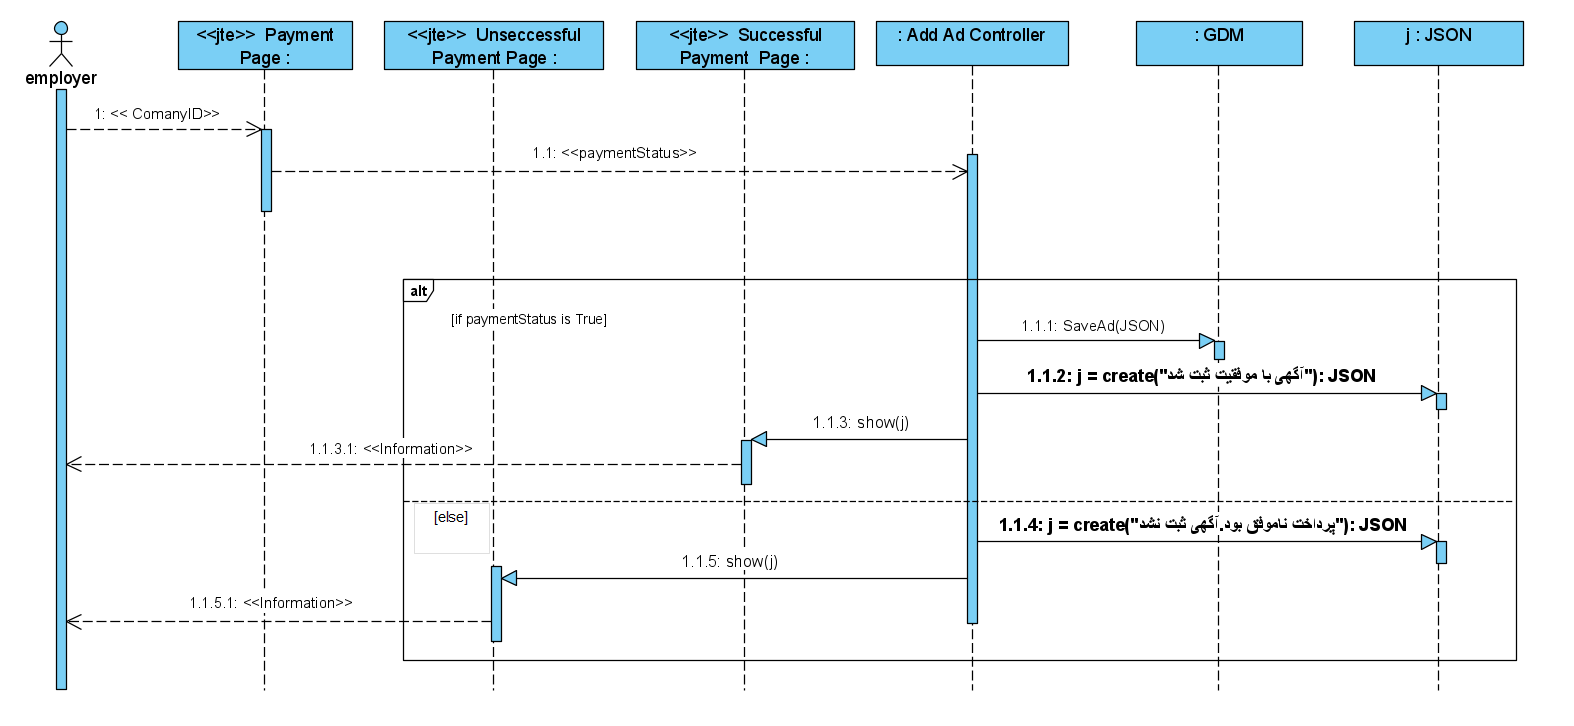
\includegraphics[width=\textwidth, angle=90, height=\textheight]{./images/sd-1}
	\end{center}
\caption{نمودار توالی \arabic{figure}}
\label{pic:sq:1}
\end{figure}

\clearpage
\section{سناریو و مدل تعامل شئ برای گام ۳ از \uc{23}}
\subsection{سناریو تعامل شئ برای \say{جست‌وجوی آگهی}}
\setcounter{MainStepCounter}{1}
\mainstep{کاربر کلید‌واژه‌ی مربوطه را در قسمت نوار جستجو وارد می‌کند.}

\beginmainstep{صفحه‌ی اصلی، عبارت جستجو را در قالب یک آبجکت \json به همراه دیگر پارامتر‌های جستجو (مثل مرتب‌سازی و فیلتر‌ها) به کنترل‌گر جستجوی آگهی می‌فرستد.}

\majorstep{کنترل‌گر جستجوی آگهی، این آبجکت \json را به \gdm ارسال می‌کند تا عبارت را در پایگاه داده جستجو کند.}

\majorstep{اگر نتیجه‌ای:}
\indent\patchstep{یافت نشد، \gdm یک آبجکت \none را به کنترل‌گر جستجوی آگهی ارسال می‌کند.}
\indent\patchstep{در غیر این صورت، تمامی آگهی‌‌های پیدا شده را به \json اصطلاحا\\ \serialize می‌کند و به کنترل‌گر جستجوی آگهی می‌فرستد.}

\majorstep{کنترل‌گر جستجوی آگهی، نتیحه را دریافت می‌کند.}

\majorstep{اگر \none بود:}
\indent\patchstep{پیغام \say{آگهی یافت نشد} را در یک آبجکت \json ذخیره و  صفحه‌ی نتایج جستجو ارسال می‌کند.}
\indent\patchstep{در غیر این صورت، آبجکت‌ \json دریافتی را به صفحه‌ی نتایج جستجو می‌فرستد.}

\majorstep{صفحه‌ی نتابج جستجو، نتایج دریافتی را به کاربر نشان می‌دهد.}
\subsection{جدول سناریو}
\begin{table}[H]
	\caption{جدول سناریو \arabic{table}}
	\begin{adjustbox}{width=\textwidth}
		\begin{tabular}{|c|c|c|c|c|}
			\hline								
			\# & فاعل & کنش فاعل & دیگرداده‌ها/اشیا & شئ‌ای که کنش روی آن انجام می‌شود \\
			\hline
			\hline
			\sstep &
			صفحه‌ی اصلی &
			ارسال می‌کند &
			آبجکت \json &
			به کنترل‌گر جستجوی آگهی \\
			\hline
			\sstep &
			کنترل‌گر جستجوی آگهی&
			ارسال می‌کند &
			آبجکت \json &
			به \gdm\\
			\hline
			\sstep &
			\multicolumn{4}{|r|}{اگر نتیجه‌ای یافت نشد}\\
			\hline
			\sstep &
			\gdm&
			ارسال می‌کند &
			آبجکت \none&
			به کنترل‌گر جستجوی آگهی \\
			\hline
			\sstep &
			\multicolumn{4}{|r|}{در غیر این صورت}\\
			\hline
			\sstep &
			\gdm&
			\serialize می‌کند&
			آبجکت‌های پیدا شده &
			به \json \\
			\hline
			\sstep &
			\gdm &
			ارسال ‌می‌کند&
			آبجکت \json &
			به کنترل‌‌گر جستجوی آگهی \\
			\hline
			\sstep &
			کنترل‌‌گر جستجوی آگهی&
			دریافت می‌کند &
			\begin{inparaitem}
				\item \none 
			\end{inparaitem}
			یا 
			\begin{inparaitem}
				\item \json
			\end{inparaitem}
			&
			\\
			\hline
			\sstep &
			\multicolumn{4}{|r|}{اگر \none بود}
			\\
			\hline
			\sstep &
			کنترل‌گر جستجوی آگهی &
			ذخیره می‌کند &
			پیغام \say{آگهی‌ای پیدا نشد}&
			در آبجکت \json \\
			\hline
			\sstep &
			کنترل‌گر جستجوی آگهی &
			ارسال می‌کند &
			آبجکت \json &
			صفحه‌ی نتایج جستجو\\
			\hline
			\sstep &
			\multicolumn{4}{|r|}{در غیر این صورت}
			\\
			\hline
			\sstep &
			کنترل‌گر جستجوی آگهی&
			ارسال می‌کند &
			آبجکت \json دریافتی از \gdm&
			صفحه‌ی نتایج جستجو\\
			\hline
			\sstep & 
			صفحه‌ی نتایج جستجو &
			نشان می‌دهد & 
			 اطلاعات دریافتی & 
			 \\
			 \hline
		\end{tabular}
	\end{adjustbox}
\end{table}
\setcounter{MainStepCounter}{0}
\setcounter{SenarioCounter}{0}
\subsection{نمودار توالی}
نمودار توالی این جدول سناریو در شکل \ref{pic:sq:2} آمده است.
\begin{figure}
	\begin{center}
		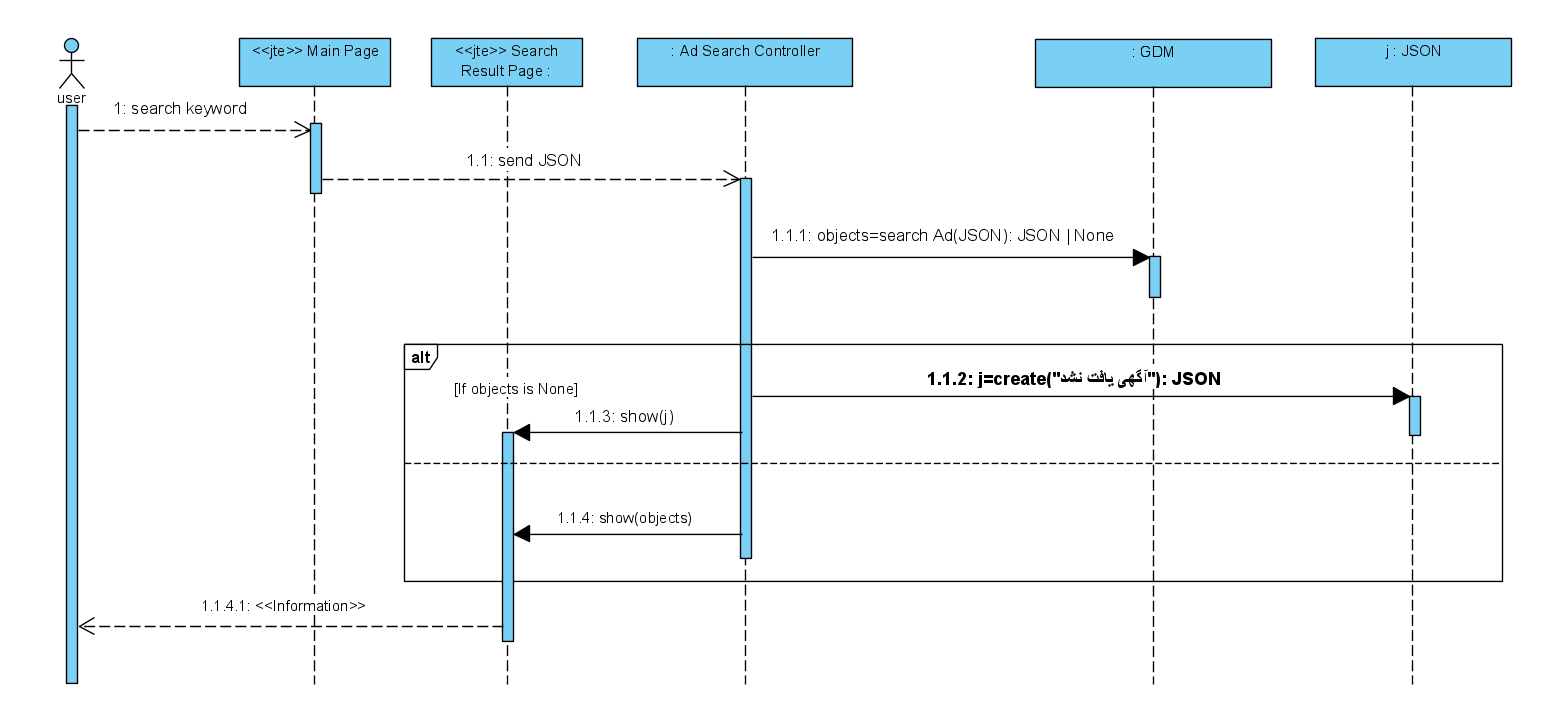
\includegraphics[width=\textwidth, angle=90, height=\textheight]{./images/sd-2}
	\end{center}
	\caption{نمودار توالی \arabic{figure}}
	\label{pic:sq:2}
\end{figure}


\clearpage
\section{سناریو و مدل تعامل شئ برای گام 2 از \uc{25}}
\subsection{سناریو تعامل شئ برای \say{مشاهده‌ی رزومه‌ها}}\label{senario-counter}
\mainstep{کارفرما بر روی دکمه‌ی \say{رزومه} در پروفایل کارجوی مدنظر کلیک می‌کند.}

\beginmainstep{صفحه‌ی پروفایل کارجو، یک درخواست مبنی بر خواست رزومه و اطلاعات کارجو را به صورت \json به کنترل‌گر مشاهده‌ی رزومه می‌فرستد.}

\majorstep{کنترل‌گر مشاهده‌ی رزومه، این اطلاعات را به \gdm می‌فرستد تا در پایگاه داده رزومه‌ را جستجو کند.}
\indent\patchstep{اگر رزومه‌ای وجود داشت، آن را در یک آبجکت \json برای کنترل‌گر مشاهده‌ی رزومه می‌فرستد.}
\indent\patchstep{اگر رزومه‌ای نبود، یک آبجکت \none به کنترل‌گر مشاهده‌ی رزومه، برمیگرداند.}

\majorstep{کنترل‌گر مشاهده‌ی رزومه، آبجکتی را دریافت می‌کند.}
\indent\patchstep{اگر پاسخ بازگشتی، \none نبود آبجکت \json را برای ارسال به صفحه‌ی پروفایل رزومه آماده نگه‌ می‌دارد.}
\indent\patchstep{در غیر این صورت، پیغام \say{عدم وجود رزومه} را در یک آبجکت \json  ذخیره می‌کند.}

\majorstep{کنترل‌گر مشاهده‌ی رزومه، آبجکت \json را به صفحه‌ی پروفایل کارجو می‌فرستد.}

\majorstep{صفحه‌ی پروفایل کارجو، اطلاعات را به کارفرما نشان می‌دهد.}
% --------------------------------------------------------
\setcounter{MainStepCounter}{0}

\subsection{جدول سناریو}
\begin{table}[H]
	\caption{جدول سناریو \arabic{table}}
	\begin{adjustbox}{width=\textwidth}
		\begin{tabular}{|c|c|c|p{0.4\textwidth}|c|}
			\hline
			\# & فاعل & کنش فاعل & دیگرداده‌ها/اشیا & شئ‌ای که کنش روی آن انجام می‌شود \\
			\hline
			\hline
			\sstep & 
			کارفرما &
			کلیک می‌کند &
			دکمه‌ی رزومه &
			از صفحه‌ی پروفایل کارجو \\
			\hline
			\sstep & 
			صفحه‌ی پروفایل کارجو &
			ارسال می‌کند &
			\begin{inparaitem}
				\item درخواست رزومه‌ی کارجو
				\item آبجکت \json اطلاعات کارجو
			\end{inparaitem} &
			به کنترل‌گر مشاهده‌ی رزومه \\
			\hline
			\sstep & 
			کنترل‌گر مشاهده‌ی رزومه &
			ارسال می‌کند &
			\json &
			به \gdm \\
			\hline
			\sstep & \multicolumn{4}{|r|}{اگر رزومه‌ای وجود داشت} \\
			\hline
			\sstep & 
			\gdm &
			ذخیره می‌کند &
			رزومه &
			در \json\\
			\hline
			\sstep & 
			\gdm &
			ارسال می‌کند &
			آبجکت \json &
			کنترل‌گر مشاهده‌ی رزومه \\
			\hline
			\sstep & \multicolumn{4}{|r|}{اگر رزومه‌ای وجود نداشت}\\
			\hline
			\sstep & 
			\gdm&
			بر می‌گرداند &
			\none&
			به کنترل‌گر مشاهده‌ی رزومه \\
			\hline
			\sstep & \multicolumn{4}{|r|}{اگر آبجکت دریافتی \none بود} \\
			\hline
			\sstep & 
			کنترل‌گر مشاهده‌ی رزومه &
			ذخیره می‌کند &
			متن \say{عدم وجود رزومه}&
			آبجکت \json\\
			\hline
			\sstep & \multicolumn{4}{|r|}{در غیر این صورت} \\
			\hline
			
			\sstep & 
			کنترل‌گر مشاهده‌ی رزومه &
			ارسال می‌کند &
			آبجکت \json رزومه &
			به صفحه‌ی پروفایل کارجو \\
			\hline
			\sstep &
			صفحه‌ی نمایش رزومه &
			نمایش می‌دهد &
			اطلاعات دریافتی &
			\\
			\hline
		\end{tabular}
	\end{adjustbox}
\end{table}
\setcounter{MainStepCounter}{0}
\setcounter{SenarioCounter}{0}
\subsection{نمودار توالی}
نمودار توالی این جدول سناریو در شکل \ref{pic:sq:3} آمده است.
\begin{figure}
	\begin{center}
		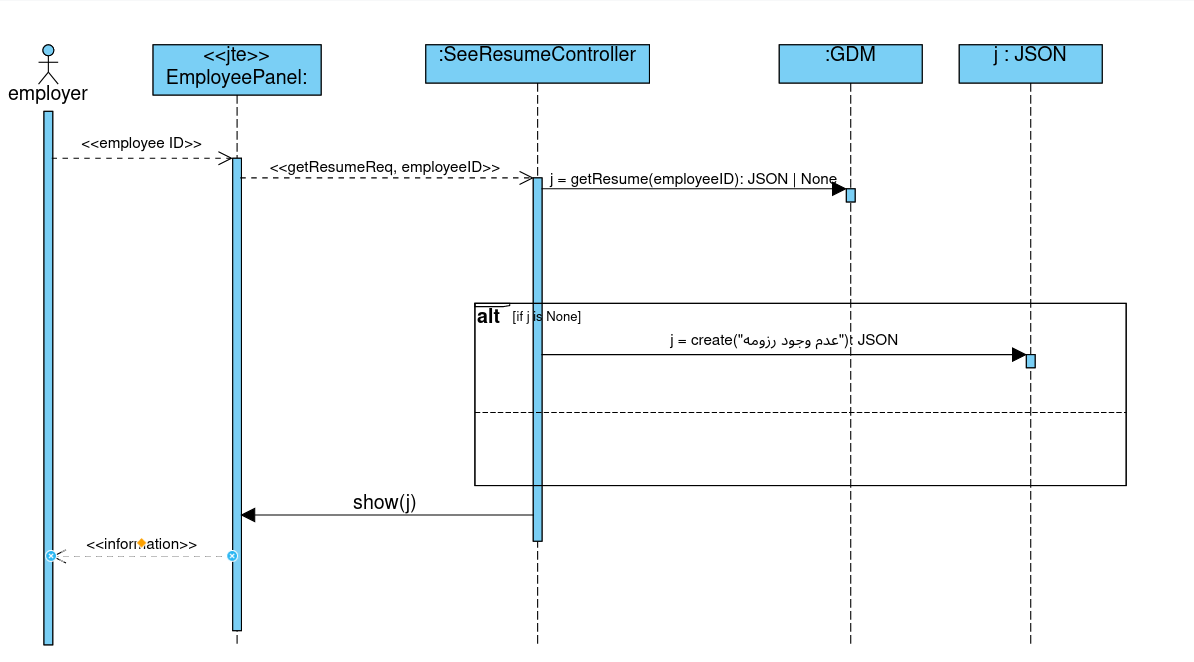
\includegraphics[width=\textwidth, angle=90, height=\textheight]{./images/sd-3}
	\end{center}
	\caption{نمودار توالی \arabic{figure}}
	\label{pic:sq:3}
\end{figure}

\clearpage
\section{سناریو و مدل تعامل شئ برای گام 2 از \uc{17}}
\subsection{سناریو تعامل شئ برای \say{نشان‌دار کردن آگهی}}
\mainstep{کارجو روی علامت ستاره در صفحه‌ی مربوط به آگهی مدنظر کلیک می‌کند.}

\beginmainstep{صفحه‌ی آگهی، اطلاعات مربوط به آگهی، کارجو و درخواستی مبنی بر نشان‌دار کردن این آگهی را با یک آبجکت \json به کنترل‌گر نشان‌دار کردن آگهی ارسال می‌کند.}

\majorstep{کنترل‌گر نشان‌دار کردن آگهی از \gdm آبجکت کارجو را درخواست می‌کند.}

\majorstep{کنترل‌گر نشان‌دار کردن آگهی بررسی می‌کند که آیا این آگهی جزو آگهی‌های نشان‌دار شده‌ی این آبجکت کارجو هست یا خیر.}
\indent\patchstep{اگر آگهی جزو آگهی‌های نشان‌دار بود:}
\indent\indent\betastep{آن را از آگهی‌های نشان‌دار کارجو حذف می‌کند.}
\indent\indent\betastep{کنترل‌گر نشان‌دار کردن آگهی پیغام \say{آگهی از آگهی‌های نشان‌دار حذف شد.} را در یک آبجکت \json ذخیره می‌کند.}
\indent\patchstep{در غیر این صورت:}
\indent\indent\betastep{آن را به آگهی‌های نشان‌دار کارجو می‌افزاید.}
\indent\indent\betastep{کنترل‌گر نشان‌دار کردن آگهی، پیغام \say{آگهی به آگهی‌های نشان‌دار افزوده شد.} را در یک آبجکت \json ذخیره می‌کند.}

\majorstep{کنترل‌گر نشان‌دار کردن آگهی، آبجکت کارجو را به \gdm می‌فرستد.}

\majorstep{\gdm آن را در پایگاه داده ذخیره می‌کند.}

\majorstep{کنترل‌گر، آبجکت \json را به صفحه‌ی آگهی ارسال می‌کند.}

\majorstep{صفحه‌ی آگهی، اطلاعات دریافتی را به کارجو نشان می‌دهد.}
\subsection{جدول سناریو}
\begin{table}[H]
	\caption{جدول سناریو \arabic{table}}
	\begin{adjustbox}{width=\textwidth}
		\begin{tabular}{|c|c|c|p{6cm}|c|}
			\hline											
			\# & فاعل & کنش فاعل & دیگرداده‌ها/اشیا & شئ‌ای که کنش روی آن انجام می‌شود \\
			\hline
			\hline
			\sstep &
			کارجو &
			کلیک می‌کند &
			دکمه‌ی ستاره &
			در صفحه‌ی آگهی \\
			\hline
			\sstep &
			صفحه‌ی آگهی &
			ارسال می‌کند &
			\begin{inparaitem}
				\item آگهی 
				\item کارجو
				\item درخواستی مبنی بر نشان‌دار کردن
			\end{inparaitem}
			&
			به کنترل‌گر نشان‌دار کردن آگهی \\
			\hline
			\sstep &
			کنترل‌گر نشان‌دار کردن آگهی &
			درخواست می‌کند &
			آبجکت کارجو &
			از \gdm \\
			\hline
			\sstep &
			\gdm &
			ارسال می‌کند &
			آبجکت کارجو &
			به کنترل‌گر نشان‌دار کردن آگهی \\
			\hline
			\sstep &
			کنترل‌گر نشان‌دار کردن آگهی &
			بررسی می‌کند &
			آگهی &
			در آبجکت کارجو \\
			\hline
			\sstep &
			\multicolumn{4}{|r|}{اگر آگهی در لیست آگهی‌های نشان‌دار بود:}\\
			\hline
			\sstep &
			کنترل‌گر نشان‌دار کردن آگهی &
			حذف می‌کند &
			آگهی‌&
			از لیست آگهی‌های نشان‌دار کارجو \\
			\hline
			\sstep &
			کنترل‌گر نشان‌دار کردن آگهی &
			ذخیره می‌کند &
			پیغام \say{آگهی‌ از آگهی‌های نشان‌دار حذف شد.}&
			در آبجکت \json \\
			\hline
			\sstep &
			\multicolumn{4}{|r|}{در غیر این صورت}\\
			\hline
			\sstep &
			کنترل‌گر نشان‌دار کردن آگهی &
			اضافه می‌کند &
			آگهی‌ &
			به لیست آگهی‌های نشان‌دار کارجو \\
			\hline
			\sstep &
			کنترل‌گر نشان‌دار کردن آگهی &
			ذخیره می‌کند &
			پیغام \say{آگهی‌ به آگهی‌های نشان‌دار افزوده شد.}&
			در آبجکت \json \\
			\hline
			\sstep &
			کنترل‌گر نشان‌دار کردن آگهی &
			ارسال می‌کند &
			آبجکت کارجو &
			به \gdm \\
			\hline
			\sstep &
			کنترل‌گر نشان‌دار کردن آگهی &
			ارسال می‌کند &
			آبجکت \json &
			به صفحه‌ی آگهی\\
			\hline
						\sstep &
			صفحه‌ی آگهی &
			نشان می‌دهد &
			اطلاعات دریافتی &
			\\
			\hline
			
		\end{tabular}
	\end{adjustbox}
\end{table}
\setcounter{MainStepCounter}{0}
\setcounter{SenarioCounter}{0}
\subsection{نمودار توالی}
نمودار توالی این جدول سناریو در شکل \ref{pic:sq:4} آمده است.
\begin{figure}
	\begin{center}
		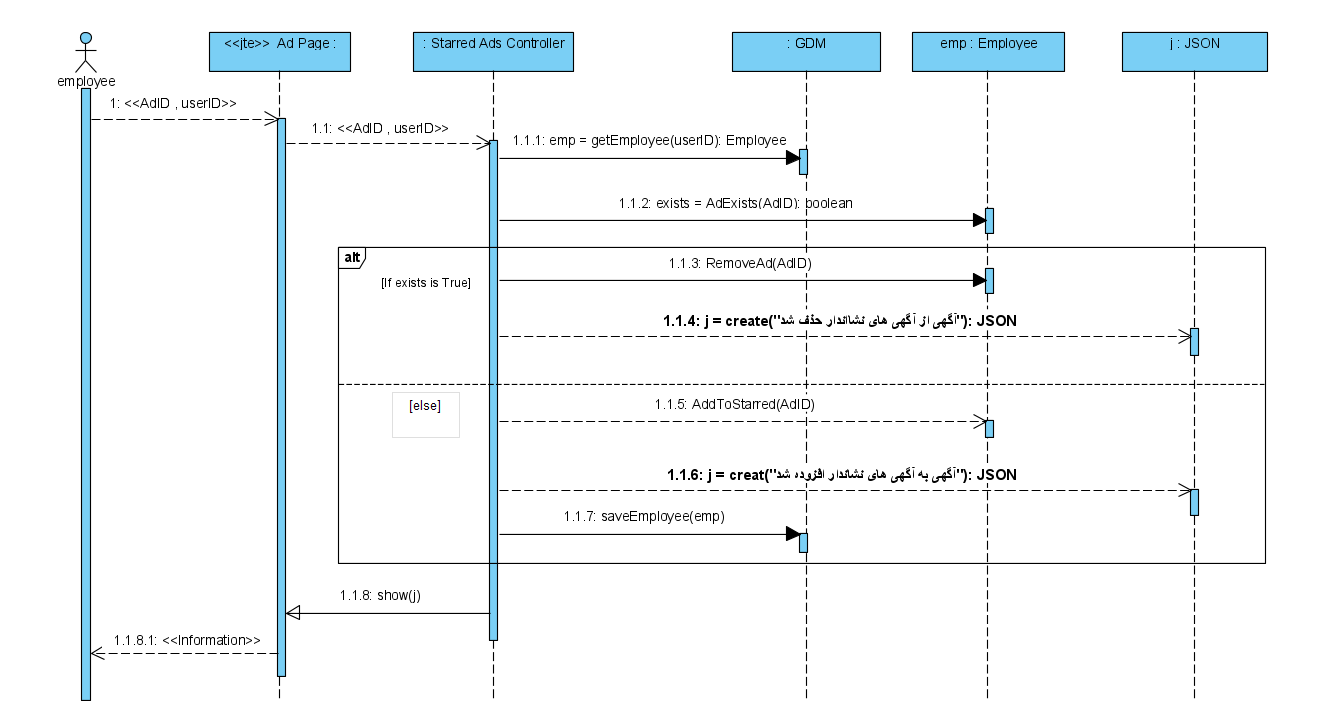
\includegraphics[width=\textwidth, angle=90, height=\textheight]{./images/sd-4}
	\end{center}
	\caption{نمودار توالی \arabic{figure}}
	\label{pic:sq:4}
\end{figure}

\clearpage
\section{سناریو و مدل تعامل شئ برای گام 2 از \uc{18}}
\subsection{سناریو تعامل شئ برای \say{مشاهده‌ی وضعیت آگهی‌های درخواستی}}
\mainstep{کارجو روی دکمه‌ی \say{وضعیت آگهی‌های درخواستی} در قسمت نوارابزار پنل کاربری کارجو کلیک می‌کند.}

\beginmainstep{صفحه‌ی پنل کاربری، درخواستی مبنی بر آگهی‌های درخواستی کارجو را به کنترل‌گر آگهی‌های درخواستی ارسال می‌کند.}

\majorstep{کنترل‌گر آگهی‌های درخواستی، شئ مربوط به آگهی‌‌های درخواستی را از \gdm درخواست می‌کند.}

\majorstep{\gdm شئ /اشیاء مربوط به آگهی‌های درخواستی را از پایگاه داده‌ می‌خواند.}
\indent\patchstep{اگر شئ‌ای موجود نباشد:}
\indent\indent\betastep{\gdm یک آبجکت \none ایجاد می‌کند.}
\indent\indent\betastep{\gdm شئ ساخته شده را به کنترل‌گر آگهی‌های درخواستی می‌فرستد.}
\indent\patchstep{اگر شئ/اشیاء مربوط به آگهی‌های درخواستی موجود باشد:}
\indent\indent\betastep{\gdm نتایج را در یک آبجکت \json ذخیره و به کنترل‌گر آگهی‌های درخواستی می‌فرستد.}

\majorstep{کنترل‌گر آگهی‌های درخواستی یک آبجکت \json یا \none دریافت می‌کند}
\indent\patchstep{اگر آبجکت \none بود:}
\indent\indent\betastep{کنترل‌گر آگهی‌های درخواستی پیغام \say{آگهی‌ درخواستی‌ای موجود نمی‌باشد} را در یک آبجکت \json ذخیره می‌کند.}

\majorstep{کنترل‌گر آگهی‌های درخواستی، آبجکت \json را به صفحه‌ی پنل کارجو ارسال ‌می‌کند.}

\subsection{جدول سناریو}
\begin{table}[H]
	\caption{جدول سناریو \arabic{table}}
	\begin{adjustbox}{width=\textwidth}
		\begin{tabular}{|c|c|c|c|c|}
			\hline					
			\# & فاعل & کنش فاعل & دیگرداده‌ها/اشیا & شئ‌ای که کنش روی آن انجام می‌شود \\
			\hline
			\hline
			\sstep &
			کارجو &
			کلیک می‌کند &
			دکمه‌ی \say{وضعیت آگهی‌های درخواستی}&
			در قسمت پنل کارجو \\
			\hline
			\sstep &
			صفحه‌ی پنل کاربری &
			ارسال می‌کند &
			درخواست مبنی بر آگهی‌های درخواستی کارجو &
			به کنترل‌گر آگهی‌های درخواستی \\
			\hline
			\sstep &
			کنترل‌گر آگهی‌های درخواستی &
			درخواست می‌کند &
			شئ/اشیاء مربوط به آگهی‌های درخواستی &
			از \gdm\\
			\hline
			\sstep &
			\gdm &
			می‌خواند &
			شئ/اشیاء مربوط به آگهی‌های درخواستی &
			پایگاه داده \\
			\hline
			\sstep &
			\multicolumn{4}{|r|}{اگر شئ/اشیاء موجود نباشد}\\
			\hline
			\sstep &
			\gdm &
			ایجاد می‌کند &
			\none &
			\\
			\hline
			\sstep &
			\gdm &
			ارسال می‌کند &
			\none &
			به کنترل‌گر آگهی‌های درخواستی \\
			\hline
			\sstep &
			\multicolumn{4}{|r|}{اگر شئ/اشیاء وجود داشت} \\
			\hline
			\sstep &
			\gdm &
			ارسال می‌کند &
			آبجکت \json مربوط به آگهی‌های درخواستی &
			به کنترل‌گر آگهی‌های درخواستی\\
			\hline
			\sstep &
			کنترل‌گر آگهی‌های درخواستی &
			دریافت می‌کند &
			\none یا \json &
			از \gdm \\
			\hline
			\sstep &
			\multicolumn{4}{|r|}{اگر شئ \none بود}\\
			\hline
			\sstep &
			کنترل‌گر آگهی‌های درخواستی &
			ذخیره می‌کند &
			پیغام \say{درخواستی موجود نمی‌باشد.}&
			در آبجکت \json \\
			\hline
			\sstep &
			کنترل‌گر آگهی‌های درخواستی&
			ارسال می‌کند &
			آبجکت \json&
			به صفحه‌ی آگهی‌های درخواستی \\
			\hline
			\sstep &
			\multicolumn{4}{|r|}{در غیر این صورت}
			\\
			\hline
			\sstep &
			کنترل‌گر آگهی‌های درخواستی &
		    ارسال می‌کند&
			آبجکت \json دریافتی از \gdm &
			به صفحه‌ی آگهی‌های درخواستی \\
			\hline
			\sstep &
			صفحه‌ی آگهی‌های درخواستی &
			نشان می‌دهد &
			اطلاعات دریافتی &
			\\
			\hline
		\end{tabular}
	\end{adjustbox}
\end{table}
\setcounter{MainStepCounter}{0}
\setcounter{SenarioCounter}{0}
\subsection{نمودار توالی}
نمودار توالی این جدول سناریو در شکل \ref{pic:sq:5} آمده است.
\begin{figure}
	\begin{center}
		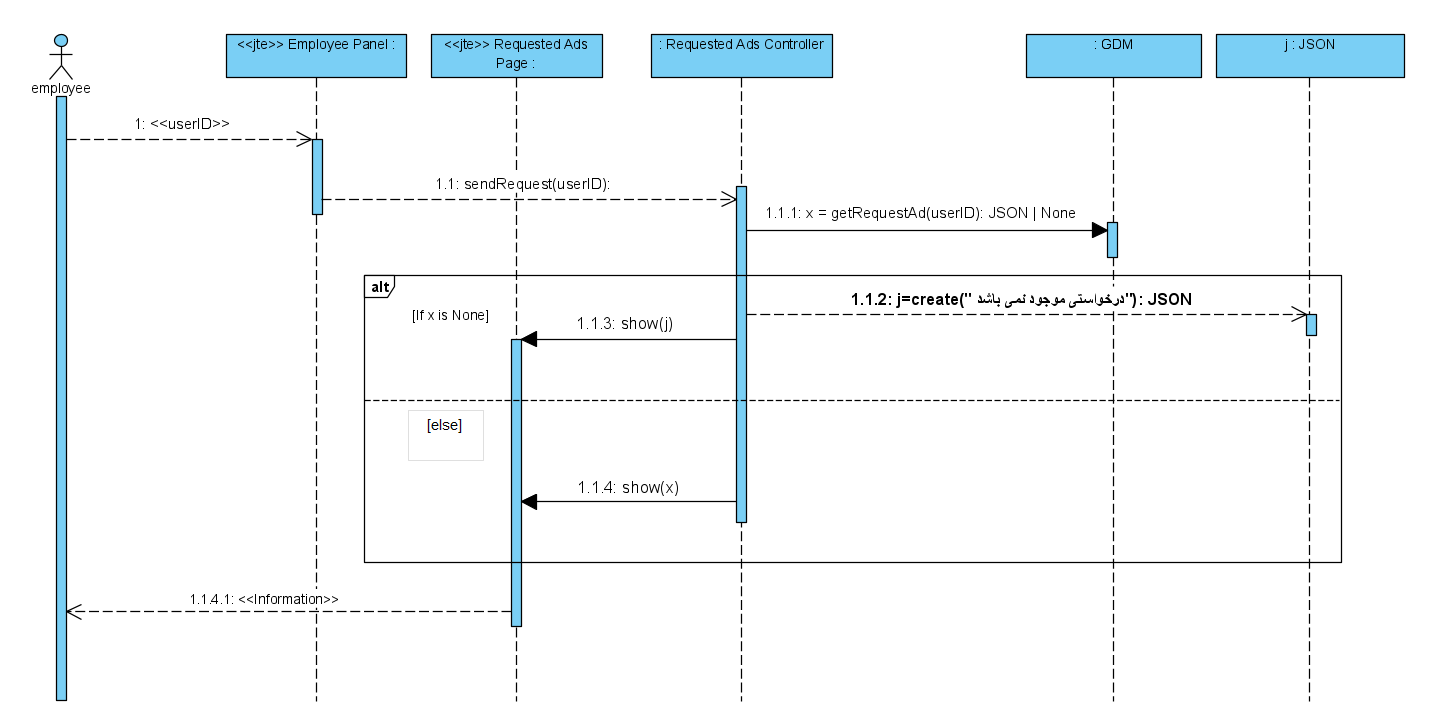
\includegraphics[width=\textwidth, angle=90, height=\textheight]{./images/sd-5}
	\end{center}
	\caption{نمودار توالی \arabic{figure}}
	\label{pic:sq:5}
\end{figure}


\clearpage
\section{سناریو و مدل تعامل شئ برای گام ۴ از \uc{12}}
\subsection{سناریو تعامل شئ برای \say{ارسال رزومه}}
\setcounter{MainStepCounter}{2}
\mainstep{کارجو رزومه‌ی خود را، بارگذاری می‌کند و به روی دکمه‌ی \say{ارسال} کلیک می‌کند.}

\beginmainstep{صفحه‌ی ارسال رزومه، فایل آپلود شده را برای کنترل‌گر ارسال رزومه می‌فرستد.
}

\majorstep{کنترل‌گر ارسال رزومه، فایل آپلود شده را بررسی می‌کند.}
\indent\patchstep{اگر فایل ارسالی، \lr{PDF} بود:}
\indent\indent\betastep{فایل را برای \gdm ارسال می‌کند تا آن را در پایگاه داده ذخیره کند.}
\indent\indent\betastep{پیغام \say{رزومه ارسال شد} را در یک آبجکت \json ذخیره می‌کند.}
\indent\indent\betastep{اطلاعات را به صفحه‌ی آگهی می‌فرستد.}
\indent\patchstep{در غیر این صورت:}
\indent\indent\betastep{پیغام \say{فرمت فایل ارسالی درست نیست، لطفا مجدداً تلاش کنید.} را در یک آبجکت \json ذخیره می‌کند.}
\indent\indent\betastep{اطلاعات را به صفحه‌ی ارسال رزومه (جهت بارگذاری مجدد) می‌فرستد.}


\subsection{جدول سناریو}
\begin{table}[H]
	\caption{جدول سناریو \arabic{table}}
	\begin{adjustbox}{width=\textwidth}
		\begin{tabular}{|c|c|c|p{6cm}|c|}
			\hline		
			\# & فاعل & کنش فاعل & دیگرداده‌ها/اشیا & شئ‌ای که کنش روی آن انجام می‌شود \\
			\hline
			\hline

			\sstep & 		
			کارجو &			
			آپلود می‌کند &			
			فایل رزومه &			
			صفحه‌ی بارگذاری رزومه \\
			\hline
			\sstep & 		
			صفحه‌ی بارگذاری رزومه &			
			ارسال می‌کند &			
			\begin{inparaitem}
				\item فایل رزومه
				\item اطلاعات کارفرما
			\end{inparaitem}
			&			
			صفحه‌ی بارگذاری رزومه\\
			\hline
			\sstep & 		
			کنترل‌گر ارسال رزومه &			
			بررسی می‌کند &			
			فایل رزومه‌ی آپلود شده &			
			\\
			\hline
			\sstep & 		
			\multicolumn{4}{|r|}{اگر فایل بارگذاری شده، \lr{PDF} بود:}\\
			\hline
			\sstep & 		
			کنترل‌گر ارسال رزومه&			
			ذخیره می‌کند &
			\begin{inparaitem}
				\item فایل رزومه
				\item اطلاعات کارفرما
			\end{inparaitem} &			
			آبجکت \json
			\\
			\hline
			\sstep & 		
			کنترل‌گر ارسال رزومه &			
			ارسال می‌کند &			
			آبجکت \json &			
			به \gdm\\
			\hline
			\sstep & 		
			کنترل‌گر ارسال رزومه&			
			ذخیره می‌کند &			
			پیغام \say{رزومه ارسال شد.} &			
			در آبجکت \json \\
			\hline
			
			\sstep & 		
    		کنترل‌گر ارسال رزومه &
			ارسال می‌کند &			
			آبجکت \json &			
			صفحه‌ی آگهی \\
			\hline
			\sstep & 		
			\multicolumn{4}{|r|}{اگر \lr{PDF} نبود:}\\
			\hline
			\sstep & 		
			کنترل‌گر ارسال رزومه&			
			ذخیره می‌کند &			
			پیغام \say{فرمت فایل ارسالی درست نیست، لطفا مجدداً تلاش کنید.}&			
			آبجکت \json \\
			\hline
			\sstep & 		
			کنترل‌گر &			
			ارسال می‌کند &			
			آبجکت \json &			
			صفحه‌ی بارگذاری رزومه \\
			\hline
		\end{tabular}
	\end{adjustbox}
\end{table}
\setcounter{MainStepCounter}{0}
\setcounter{SenarioCounter}{0}
\subsection{نمودار توالی}
نمودار توالی این جدول سناریو در شکل \ref{pic:sq:6} آمده است.
\begin{figure}
	\begin{center}
		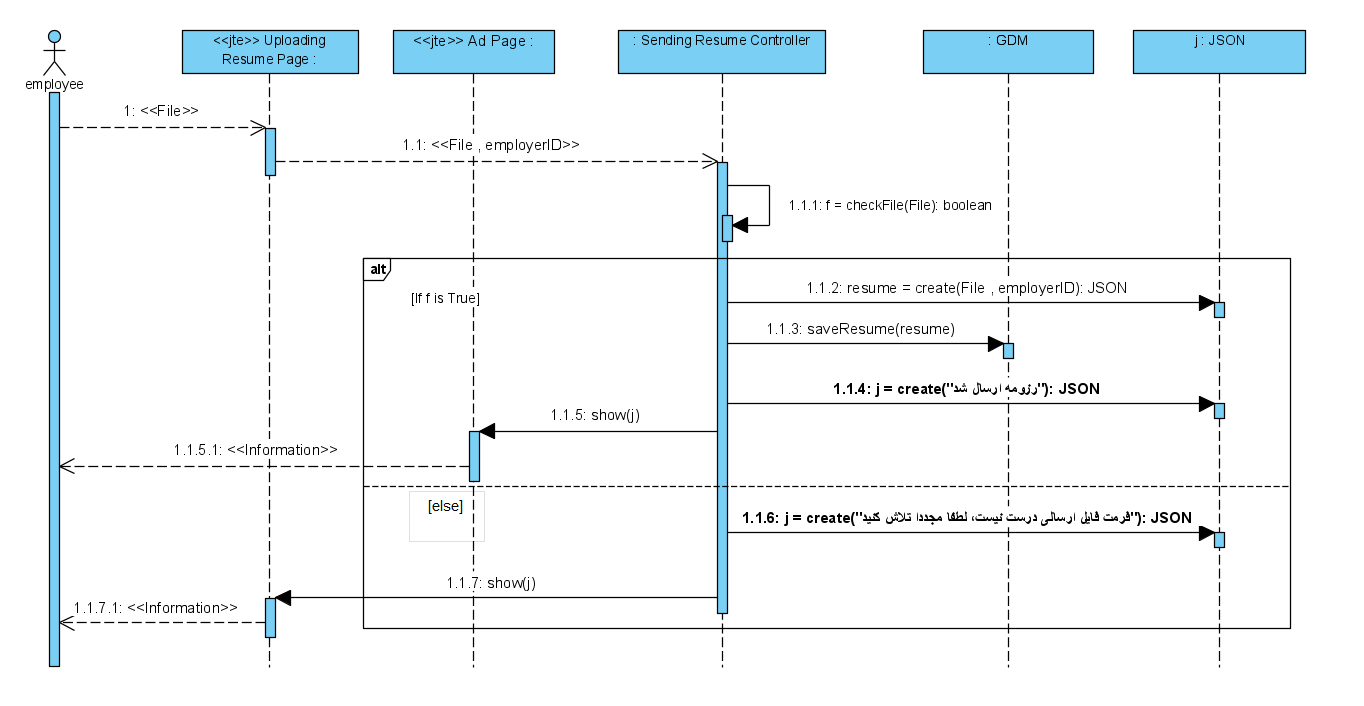
\includegraphics[width=\textwidth, angle=90, height=\textheight]{./images/sd-6}
	\end{center}
	\caption{نمودار توالی \arabic{figure}}
	\label{pic:sq:6}
\end{figure}


\clearpage
\section{سناریو و مدل تعامل شئ برای گام ۶ از \uc{1}}
\subsection{سناریو تعامل شئ برای \say{ثبت‌نام کاربر}}
\setcounter{MainStepCounter}{4}
\mainstep{کاربر اطلاعات را وارد کرده و به روی دکمه‌ی ثبت‌نام کلیک می‌کند.}

\beginmainstep{صفحه ثبت‌نام اطلاعات را به کنترل‌گر ثبت‌نام می‌فرستد.}

\majorstep{کنترل‌گر ثبت‌نام \lr{userID} دریافت شده از صفحه‌ی ثبت‌نام را به \gdm می‌فرستد.}

\majorstep{\gdm وجود این \lr{userID} را در پایگاه داده بررسی می‌کند:}
\indent\patchstep{اگر این \lr{userID} در پایگاه داده بود، \lr{True} برمی‌گرداند.\RTLfootnote{یعنی \lr{userID} در پایگاه داده وجود داشته و این \lr{userID} تکراری است.}}
\indent\indent\betastep{کنترل‌گر ثبت‌نام پیغام \say{کاربری قبلا با این آیدی ثبت‌نام کرده است.} را در یک آبجکت \json می‌نویسد.}
\indent\indent\betastep{کنترل‌گر ثبت‌نام اطلاعات را به صفحه‌ ثبت‌نام ارسال می‌کند.}

\indent\patchstep{اگر این \lr{userID} در پایگاه داده نبود، \lr{False} برمی‌گرداند.}
\indent\indent\betastep{کنترل‌گر ثبت‌نام پیغام \say{ثبت‌نام موفقیت‌آمیز بود.} را در یک آبجکت \json می‌نویسد.}
\indent\indent\betastep{کنترل‌گر ثبت‌نام اطلاعات را به \gdm ارسال می‌کند تا کاربر در پایگاه داده ثبت بشود.}

\indent\indent\betastep{اگر کاربر ثبت‌نام شده کارجو بود:}
\indent\indent\indent\alphastep{کنترل‌گر ثبت‌نام، اطلاعات پنل کاربری کارجوی تازه ثبت‌نام شده را، از \gdm درخواست می‌کند}
\indent\indent\indent\alphastep{کنترل‌گر ثبت‌نام اطلاعات را به پنل کاربری کارجو ارسال می‌کند}
\indent\indent\betastep{اگر کاربر ثبت‌نام شده کارفرما بود:}
\indent\indent\indent\alphastep{کنترل‌گر ثبت‌نام، اطلاعات پنل کاربری کار‌فرما تازه ثبت‌نام شده را، از \gdm درخواست می‌کند}
\indent\indent\indent\alphastep{کنترل‌گر ثبت‌نام اطلاعات را به پنل کاربری کارفرما ارسال می‌کند.}

\subsection{جدول سناریو}
\begin{table}[H]
	\caption{جدول سناریو \arabic{table}}
	\begin{adjustbox}{width=\textwidth}
		\begin{tabular}{|c|c|c|c|c|}
			\hline								
\# & فاعل & کنش فاعل & دیگرداده‌ها/اشیا & شئ‌ای که کنش روی آن انجام می‌شود \\
			\hline
			\hline
			\sstep &
			کاربر &
            کلیک می‌کند &
			دکمه‌ی ثبت‌نام & 
			صفحه‌ی ثبت‌نام \\
			\hline
\sstep &
صفحه‌ی ثبت‌نام & 
ارسال می‌کند &
اطلاعات صفحه‌ی ثبت‌نام &
به کنترل‌گر ثبت‌نام\\
\hline
\sstep &
کنترل‌گر ثبت‌نام &
ارسال می‌کند &
\lr{userID}&
به \gdm \\
\hline
\sstep &
\gdm &
بررسی می‌کند &
\lr{userID}&
در پایگاه داده \\
\hline
\sstep &
\multicolumn{4}{|r|}{اگر \lr{userID} در پایگاه داده بود}
\\
\hline
\sstep &
\gdm &
برمی‌گرداند &
\lr{True}&
به کنترل‌گر ثبت‌نام \\
\hline
\sstep &
کنترل‌گر ثبت‌نام &
ذخیره می‌کند &
پیغام \say{کاربری قبلا با این آیدی ثبت‌نام کرده است.}&
در آبجکت \json \\
\hline
\sstep &
کنترل‌گر ثبت‌نام &
ارسال می‌‌کند &
اطلاعات &
به صفحه‌ ثبت‌نام \\
\hline
\sstep &
\multicolumn{4}{|r|}{اگر \lr{userID} در پایگاه داده نبود}
\\
\hline
\sstep &
\gdm &
برمی‌گرداند &
\lr{False}&
به کنترل‌گر ثبت‌نام \\
\hline
\sstep &
کنترل‌گر ثبت‌نام &
ذخیره می‌کند &
پیغام \say{ثبت‌نام موفقیت‌آمیز بود.}&
در آبجکت \json \\
\hline
\sstep &
کنترل‌گر ثبت‌نام &
ارسال می‌‌کند &
اطلاعات کاربر &
به \gdm \\
\hline
\sstep &
\gdm &
ذخیره‌ می‌کند&
کاربر &
در پایگاه داده \\
\hline
\sstep &
\multicolumn{4}{|r|}{اگر کاربر ثبت‌نام شده کارجو بود}
\\
\hline
\sstep &
کنترل‌گر ثبت‌نام&
درخواست می‌کند &
اطلاعات پنل کاربری کارجو &
از \gdm \\
\hline
\sstep &
کنترل‌گر ثبت‌نام&
ارسال می‌کند &
اطلاعات پنل کاربری کارجو &
از به پنل کاربری کارجو \\
\hline
\sstep &
\multicolumn{4}{|r|}{اگر کاربر ثبت‌نام شده کارفرما بود}
\\
\hline
\sstep &
کنترل‌گر ثبت‌نام&
درخواست می‌کند &
اطلاعات پنل کاربری کارفرما &
از \gdm \\
\hline
\sstep &
کنترل‌گر ثبت‌نام&
ارسال می‌کند &
اطلاعات پنل کاربری کارفرما &
از به پنل کاربری کارفرما \\
\hline
\sstep &
پنل‌های کاربری &
نشان می‌دهند &
اطلاعات &
\\
\hline

		\end{tabular}
	\end{adjustbox}
\end{table}
\setcounter{MainStepCounter}{0}
\setcounter{SenarioCounter}{0}
\subsection{نمودار توالی}
نمودار توالی این جدول سناریو در شکل \ref{pic:sq:7} آمده است.
\begin{figure}
	\begin{center}
		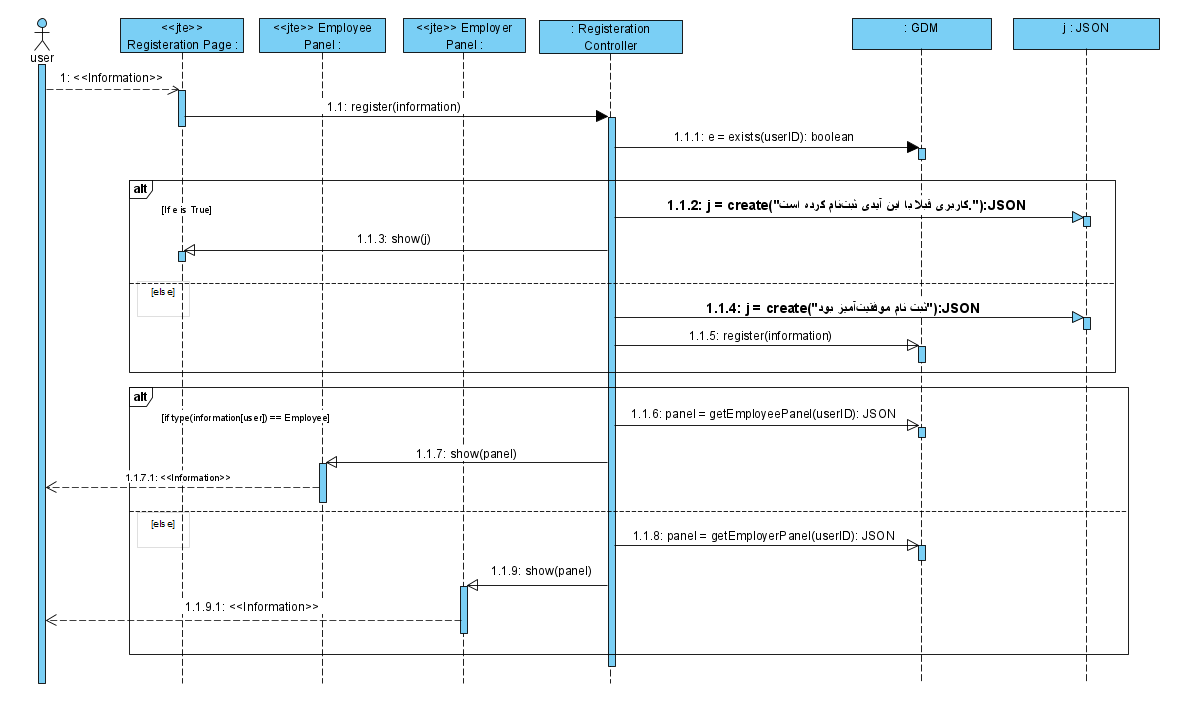
\includegraphics[width=\textwidth, angle=90, height=\textheight]{./images/sd-7}
	\end{center}
	\caption{نمودار توالی \arabic{figure}}
	\label{pic:sq:7}
\end{figure}
